\appendix
\label{Appendix - Calculations}
%================================================================
%================================================================

\chapter{Derivations for Chapter 1}
\label{app:supercond-derivation}
\section*{Derivation of the London Equation Solutions}
\label{app:london_derivation}

The London differential equation for the magnetic induction $\mathbf{B}$ inside a superconductor is a vector Helmholtz equation:
\begin{equation}
    \nabla^2 \mathbf{B} = \frac{\mathbf{B}}{\lambda_L^2} \implies \left(\nabla^2 - \frac{1}{\lambda_L^2}\right) \mathbf{B} = 0,
    \label{eq:appendix_london_helmholtz}
\end{equation}
where $\lambda_L$ is the London penetration depth. This section demonstrates the solution process for the semi-infinite planar geometry.

\paragraph{Semi-Infinite Planar Solution.}
\label{app:planar_solution}

We consider a superconductor occupying the region $x > 0$ with an external field $\mathbf{H}_0 = H_0 \hat{\mathbf{z}}$ applied parallel to the surface ($x=0$). By symmetry, the internal field $\mathbf{B}$ is uniform in $y$ and $z$ and parallel to the applied field:
$$\mathbf{B}(x) = B_z(x) \hat{\mathbf{z}}.$$\\
Substituting this form into Equation \eqref{eq:appendix_london_helmholtz} causes the vector Laplacian $\nabla^2$ to simplify to the scalar second derivative with respect to $x$:
$$\frac{d^2 B_z}{dx^2} = \frac{B_z}{\lambda_L^2}$$\\
This is a second-order linear ordinary differential equation with constant coefficients. Assuming a solution of the form $B_z(x) = e^{kx}$ yields the characteristic equation $k^2 = 1/\lambda_L^2$, leading to two roots, $k = \pm 1/\lambda_L$. The general solution for $x>0$ is:
$$B_z(x) = A e^{+x/\lambda_L} + C e^{-x/\lambda_L}$$

\paragraph{Boundary and Regularity Conditions}
The coefficients $A$ and $C$ are determined by the physical constraints:
\begin{enumerate}
    \item \textbf{Regularity at Infinity ($x \to \infty$):} For the solution to remain finite and physically represent the Meissner effect (flux expulsion), the growing exponential term must be eliminated:
    $$B_z(x) \to 0 \text{ as } x \to \infty \implies A = 0.$$
    The solution reduces to $B_z(x) = C e^{-x/\lambda_L}$.
    \item \textbf{Boundary Condition at Interface ($x = 0$):} The tangential component of the magnetic field strength ($\mathbf{H}$) is continuous across the boundary. Assuming $\mathbf{B} = \mu\mathbf{H}$ inside the superconductor:
    $$B_z(0) = \mu H_{0, \text{tangential}} = \mu H_0.$$
    Substituting this into the reduced solution:
    $$C e^{0} = \mu H_0 \implies C = \mu H_0.$$
\end{enumerate}

Substituting the coefficient $C$ back into the solution yields the field decay result:
$$\mathbf{B}(x) = \mu H_0\,e^{-x/\lambda_L}\,\hat{\mathbf{z}} = \mathbf{B}_0 \,e^{-x/\lambda_L}\,\hat{\mathbf{z}} $$


%================================================================
\chapter{Derivations for Chapter 2}
\label{app:BCS-derivation}
\section*{Fourier derivation of the Cooper integral equation}
\label{app:cooper_FT}

We start from the relative-coordinate Schr\"odinger equation for two identical electrons
(with reduced mass \(\mu=m/2\))
\begin{equation}
\left[-\frac{\hbar^2\nabla_{\mathbf r}^2}{2\mu}+V(\mathbf r)\right]\psi(\mathbf r)
=\tilde E\,\psi(\mathbf r),
\label{eq:cooper_relative_sch_app}
\end{equation}
obtained after separating centre-of-mass and relative motion in the main text.\\
We adopt
\begin{equation}
\psi(\mathbf{k})=\int d^3 r\, \psi(\mathbf r)\,e^{-i\mathbf k\cdot\mathbf r},
\qquad
\psi(\mathbf r)=\int\!\frac{d^3 k}{(2\pi)^3}\, \psi(\mathbf k)\,e^{i\mathbf k\cdot\mathbf r},
\label{eq:FT_defs_app}
\end{equation}
and similarly
\begin{equation}
    V(\mathbf q)=\int d^3r\,V(\mathbf r)\,e^{-i\mathbf q\cdot\mathbf r}.
    \label{eq:FT_defs_app2}
\end{equation}

Applying \eqref{eq:FT_defs_app} and \eqref{eq:FT_defs_app2} to \eqref{eq:cooper_relative_sch_app} gives, term by term,
\begin{align}
\mathcal{F}\!\left\{-\frac{\hbar^2}{2\mu}\nabla_{\mathbf r}^2 \psi(\mathbf r)\right\}
&= \frac{\hbar^2 k^2}{2\mu}\,\psi(\mathbf k), \nonumber \\[4pt]
\mathcal{F}\!\left\{V(\mathbf r)\psi(\mathbf r)\right\}
%&= \int\!\frac{d^3 k'}{(2\pi)^3}\, V(\mathbf k-\mathbf k')\,\psi(\mathbf k'),\\[4pt]
%\mathcal{F}\!\left\{\tilde E\,\psi(\mathbf r)\right\}
&=  E\,\psi(\mathbf k). \nonumber
\end{align}


For the second term, we recall that the Fourier transform of a product of two functions is given by the convolution of their Fourier transforms:
\[
\mathcal{F}\{f(\mathbf r)g(\mathbf r)\}(\mathbf k)
= \int\!\frac{d^3k'}{(2\pi)^3}\, f(\mathbf k-\mathbf k')\, g(\mathbf k').
\]
Applying this to \(V(\mathbf r)\psi(\mathbf r)\) gives
\[
\mathcal{F}\!\left\{V(\mathbf r)\psi(\mathbf r)\right\}
= \int\!\frac{d^3k'}{(2\pi)^3}\, V(\mathbf k-\mathbf k')\, \psi(\mathbf k').
\]

Collecting all terms gives:
\begin{equation}
\left(\frac{\hbar^2 k^2}{2\mu}\right)\psi(\mathbf k)
+\int\!\frac{d^3 k'}{(2\pi)^3}\, V(\mathbf k-\mathbf k')\,\psi(\mathbf k')
=\tilde E\,\psi(\mathbf k).
\label{eq:momentum_schro_app}
\end{equation}
For two identical electrons: \[\mu=\frac{\mu}{2} ,\quad \implies \quad \frac{\hbar^2 k^2}{2\mu}=\frac{\hbar^2 k^2}{m}\equiv 2\epsilon_{\mathbf k}\, ,\quad  
\epsilon_{\mathbf k}=\frac{\hbar^2 k^2}{2m}.\]
\noindent Rearranging \eqref{eq:momentum_schro_app} yields the \emph{Cooper integral equation}:
\begin{equation}
\boxed{
\bigl( E-2\epsilon_{\mathbf k}\bigr)\,\psi(\mathbf k)
=\int\!\frac{d^3 k'}{(2\pi)^3}\, V(\mathbf k-\mathbf k')\,\psi(\mathbf k')}\, .
\label{eq:cooper_integral_app}
\end{equation}

Define the modified wavefunction
\[
\Delta(\mathbf k)\equiv \bigl(E-2\epsilon_{\mathbf k}\bigr)\,\psi(\mathbf k),
\qquad (E\equiv \tilde E\ \text{for }\mathbf K=0),
\]
to express \eqref{eq:cooper_integral_app} as:
\begin{equation}
\boxed{
\Delta(\mathbf k) = -\!\int\!\frac{d^3 k'}{(2\pi)^3}\;
\frac{V(\mathbf k-\mathbf k')}{\,2\epsilon_{\mathbf k'}-E\,}\;\Delta(\mathbf k')}\, .
\label{eq:cooper_Delta_app}
\end{equation}
Equations \eqref{eq:cooper_integral_app}–\eqref{eq:cooper_Delta_app} represent the Schrödinger equation for the relative motion written in momentum space.
%================================================================

%================================================================
%================================================================
%================================================================
\chapter{Derivations for Chapter 3}
\label{app:BEC-derivation}
\section*{Density of States in Three Dimensions}
\label{density_of_states}

We aim to calculate the density of states \( D(\varepsilon) \), defined as the number of available single–particle states per unit energy, as a function of the energy \( \varepsilon \).

The first step consists in counting the number of allowed states in \(k\)–space for free particles confined in a box of side \(L\) and volume \(V = L^3\), assuming periodic boundary conditions.  
Each quantum state corresponds to a point in \(k\)–space separated from the next by an interval
\[
\Delta k_x = \Delta k_y = \Delta k_z = \frac{2\pi}{L},
\]
so that the elementary volume occupied by one state in \(k\)–space is
\[
\Delta V_k = \left(\frac{2\pi}{L}\right)^3 = \frac{(2\pi)^3}{V}.
\]
Thus, the number of available states in a region of volume \( dV_k \) of \(k\)–space is given by
\[
dN = \frac{1}{\frac{(2\pi)^3}{V}}\,dV_k =  \frac{V}{(2\pi)^3}\,dV_k .
\]
 
The number of \(k\)–states within a spherical shell of radius \(k\) and thickness \(dk\) is proportional to the surface area of the sphere times \(dk\):
\[
dV_k = 4\pi k^2\,dk.
\]
Substituting into the previous expression gives
\[
dN = \frac{V}{(2\pi)^3}\,4\pi k^2\,dk = \frac{V k^2}{2\pi^2}\,dk.
\]

Differentiating the dispersion relation \( \varepsilon = \frac{\hbar^2 k^2}{2m} \), we obtain
\[
d\varepsilon = \frac{\hbar^2 k}{m}\,dk,
\qquad \text{or equivalently} \qquad
dk = \frac{m}{\hbar^2 k}\,d\varepsilon.
\]
Replacing \( dk \) in the expression for \( dN \) yields
\[
dN = \frac{V k^2}{2\pi^2} \cdot \frac{m}{\hbar^2 k}\,d\varepsilon
= \frac{V m k}{2\pi^2 \hbar^2}\,d\varepsilon.
\]

We can express the wavevector magnitude in terms of the particle energy using
\[
k = \sqrt{\frac{2m\varepsilon}{\hbar^2}}.
\]
Substituting this into the previous relation, the density of states per unit energy is obtained as
\begin{equation}
D_{3D}(\varepsilon) = \frac{dN}{d\varepsilon}
= \frac{V}{4\pi^2} \left(\frac{2m}{\hbar^2}\right)^{3/2} \varepsilon^{1/2}.
\end{equation}

\begin{figure}[H]
    \centering
    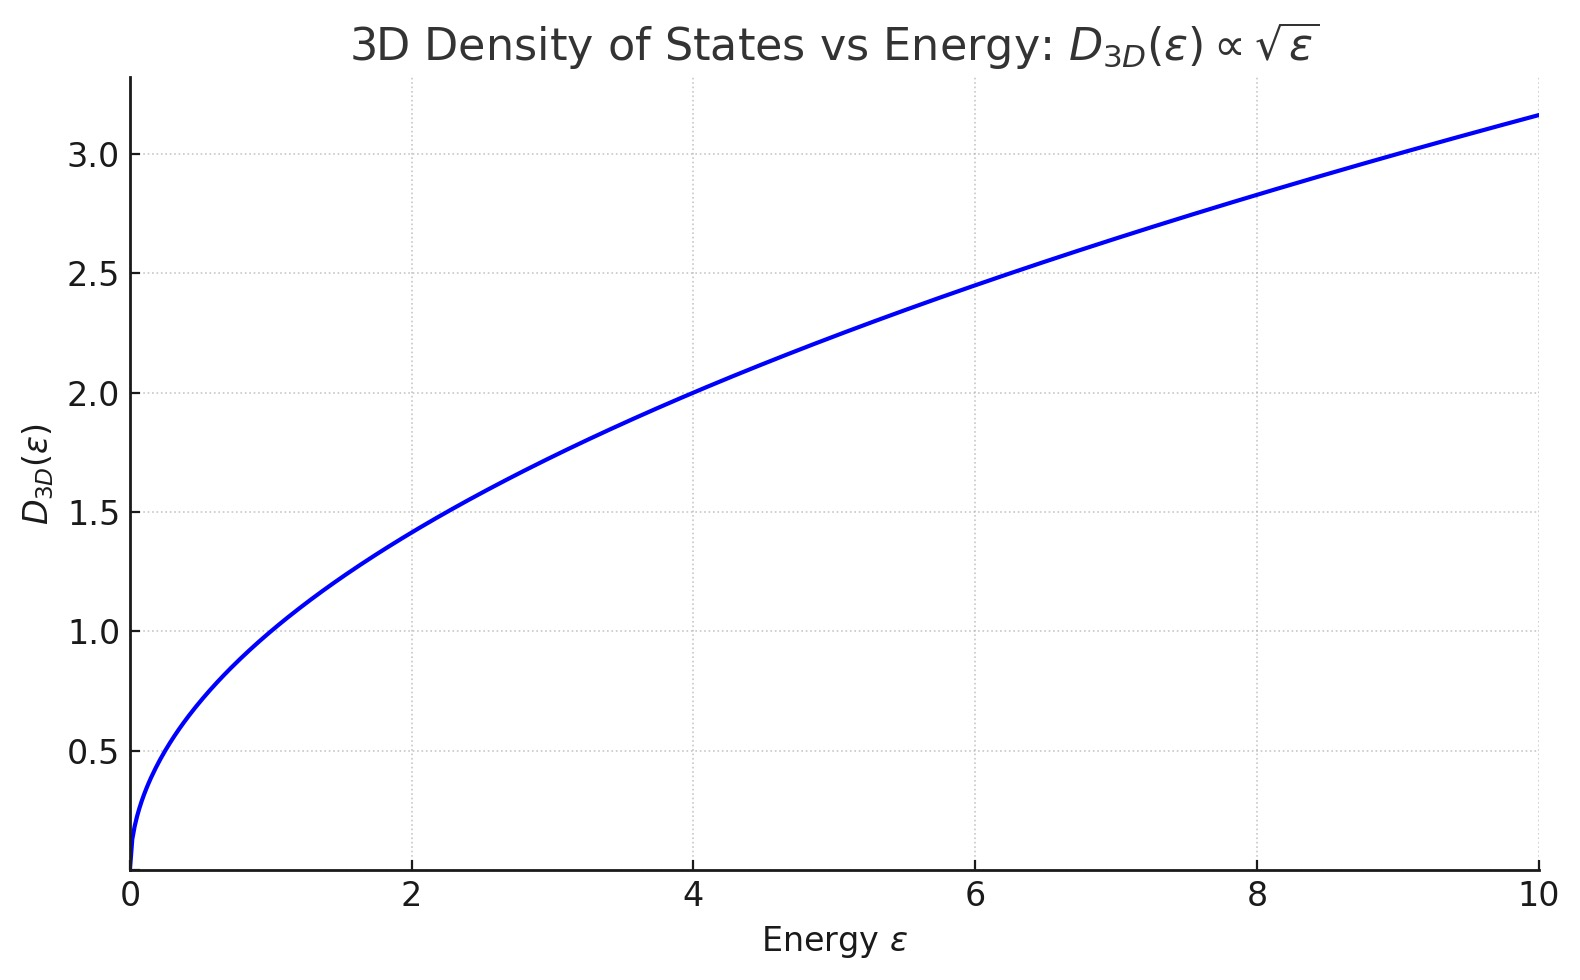
\includegraphics[scale= 0.2]{Chapters/Chapter_2/Images/3_3D.jpg}
    \caption{3D density of states $D_{3D}(\varepsilon)$ as a function of the energy.}
    \label{Figure 5 - DOS}
\end{figure}
%================================================================
\section*{Gamma function and Riemann zeta function}
\label{appendix:gamma_riemann}

In the derivation of the critical density and temperature for Bose--Einstein condensation, two special mathematical functions appear naturally: the \textit{Gamma function} and the \textit{Riemann zeta function}.  
Their properties allow one to evaluate integrals of the type
\[
    \int_0^{\infty} \frac{x^{\alpha - 1}}{e^x - 1}\, dx.
\]

\paragraph{The Gamma Function}

The Gamma function \( \Gamma(\alpha) \) generalizes the factorial function to real and complex arguments.  
It is defined for \( \Re(\alpha) > 0 \) by
\begin{equation}
    \Gamma(\alpha) = \int_0^{\infty} t^{\alpha - 1} e^{-t}\, dt.
    \label{eq:gamma_def}
\end{equation}
It satisfies the recurrence relation
\[
    \Gamma(\alpha + 1) = \alpha\, \Gamma(\alpha),
\]
and for integer values \( n \), it reduces to the factorial:
\[
    \Gamma(n) = (n - 1)!.
\]
Some useful values are
\[
    \Gamma\!\left(\tfrac{1}{2}\right) = \sqrt{\pi},
    \qquad
    \Gamma\!\left(\tfrac{3}{2}\right) = \tfrac{1}{2}\sqrt{\pi}.
\]
The Gamma function often appears in statistical physics when transforming integrals over momentum or energy to integrals over dimensionless variables.

\paragraph{The Riemann Zeta Function}

The Riemann zeta function \( \zeta(\alpha) \) is defined for \( \Re(\alpha) > 1 \) as the infinite series
\begin{equation}
    \zeta(\alpha) = \sum_{n=1}^{\infty} \frac{1}{n^{\alpha}}.
    \label{eq:zeta_def}
\end{equation}
It can also be expressed as:
\begin{equation}
    \zeta(\alpha) = \frac{1}{\Gamma(\alpha)} \int_0^{\infty} \frac{x^{\alpha - 1}}{e^x - 1}\, dx.
\end{equation}
This representation connects \( \zeta(\alpha) \) to integrals encountered in quantum statistics, particularly in the evaluation of thermodynamic quantities for Bose and Fermi gases.

For the case relevant to Bose--Einstein condensation, \( \alpha = 3/2 \), the value is
\[
    \zeta\!\left(\tfrac{3}{2}\right) \approx 2.612.
\]
Combining this with \( \Gamma(3/2) = \tfrac{\sqrt{\pi}}{2} \), the integral
\[
    \int_0^{\infty} \frac{x^{1/2}}{e^x - 1}\, dx
\]
can be evaluated as
\[
    \Gamma\!\left(\tfrac{3}{2}\right) \zeta\!\left(\tfrac{3}{2}\right)
    = \frac{\sqrt{\pi}}{2}\, \zeta\!\left(\tfrac{3}{2}\right)
    \approx 2.315.
\]
This numerical factor directly determines the prefactor in the expression for the critical density and critical temperature of the Bose gas [Eq.~\eqref{eq:nc_result}].

%================================================================
%================================================================
%================================================================
\chapter{Derivations for Chapter 4}
\label{app:BCS_BEC-derivation}
\section*{Critical Temperature for Linear Dispersion}
\label{app:Tc_linear_dispersion}

Starting from the general expression for the critical temperature of a Bose gas with dispersion relation
\[
\varepsilon_K = C_s K^s,
\]
the condensation temperature in \(d\) spatial dimensions is given by Eq.~\eqref{eq:Tc_general_1}:
\begin{equation}
T_c = \frac{C_s}{k_B}
\left[
    \frac{s\, \Gamma(d/2)\, (2\pi)^d\, n_B}
         {2\, \pi^{d/2}\, \Gamma(d/s)\, g_{d/s}(1)}
\right]^{s/d}.
\label{eq:app_Tc_general}
\end{equation}

To obtain the expression corresponding to a \textit{linear dispersion}, we set
\[
s = 1, \qquad \varepsilon_K = \alpha(d)\,\hbar v_F\, K,
\]
where \(\alpha(d)\) is a dimension-dependent numerical factor (\(\alpha(2) = 2/\pi\), \(\alpha(3) = 1/2\)) and \(v_F\) the Fermi velocity.  
Substituting these values into Eq.~\eqref{eq:app_Tc_general}, we find:
\begin{align}
T_c 
&= \frac{\alpha(d)\, \hbar v_F}{k_B}
\left[
    \frac{1 \cdot \Gamma(d/2)\, (2\pi)^d\, n_B}
         {2\, \pi^{d/2}\, \Gamma(d)\, g_d(1)}
\right]^{1/d} \nonumber \\[6pt]
&= \frac{\alpha(d)\, \hbar v_F}{k_B}
\left[
    \frac{\pi^{(d+1)/2}\, n_B}
         {\Gamma\!\left[(d+1)/2\right]\, g_d(1)}
\right]^{1/d}.
\label{eq:app_Tc_linear_final}
\end{align}

Equation~\eqref{eq:app_Tc_linear_final} reproduces Eq.~\eqref{eq:Tc_linear_dispersion} in the main text.  
This result shows that for linear dispersion (\(s=1\)), the critical temperature remains finite for all \(d > 1\), thereby explaining the possibility of condensation, and hence superconductivity, in quasi-two-dimensional systems.
%================================================================
%================================================================

\section*{Recovery of the Conventional 3D Bose–Einstein Critical Temperature}
\label{d3s2}
For a quadratic dispersion \(\varepsilon_K=C_2 K^2\) with \(C_2=\hbar^2/(2M)\) and in \(d=3\) dimensions, Eq.~\eqref{eq:Tc_general_2} gives
\[
T_c \;=\; \frac{C_2}{k_B}
\left[
\frac{s\,\Gamma\!\left(\frac d2\right) (2\pi)^d n_B}
{2\,\pi^{d/2}\,\Gamma\!\left(\frac{d}{s}\right)\,\zeta\!\left(\frac{d}{s}\right)}
\right]^{s/d}
\;=\;
\frac{\hbar^2}{2 M k_B}
\left[
\frac{2\,\Gamma\!\left(\tfrac{3}{2}\right) (2\pi)^3 n_B}
{2\,\pi^{3/2}\,\Gamma\!\left(\tfrac{3}{2}\right)\,\zeta\!\left(\tfrac{3}{2}\right)}
\right]^{2/3}.
\]
Cancelling the \(\Gamma\!\left(\tfrac{3}{2}\right)\) factor yields
\[
\text{bracket}
=
\frac{2\,\Gamma\!\left(\tfrac{3}{2}\right)\, 8\pi^3\, n_B}
     {2\,\pi^{3/2}\,\Gamma\!\left(\tfrac{3}{2}\right)\,\zeta(3/2)}
=
\frac{8\pi^3\, n_B}{\pi^{3/2}\,\zeta(3/2)}
=
\frac{8\,\pi^{3/2}\, n_B}{\zeta(3/2)}.
\]
Raising to the power \(2/3\) gives
\[
\left(\frac{8\,\pi^{3/2}\, n_B}{\zeta(3/2)}\right)^{2/3}
= 8^{2/3}\,\pi^{(3/2)\cdot(2/3)} \left(\frac{n_B}{\zeta(3/2)}\right)^{2/3}
= 4\,\pi \left(\frac{n_B}{\zeta(3/2)}\right)^{2/3}.
\]
Therefore,
\[
T_c
= \frac{\hbar^2}{2 M k_B}\, 4\pi \left(\frac{n_B}{\zeta(3/2)}\right)^{2/3}
= \frac{2\pi \hbar^2}{M k_B}\,
\left[\frac{n_B}{\zeta(3/2)}\right]^{2/3},
\]
which is Eq.~\eqref{eq:Crit_T} (identifying \(n_B \equiv n\) and $M = 2m$).

%================================================================
%================================================================
%================================================================
%========================================================
% Appendix: Variational derivation of the GL equations
%========================================================
\chapter{Derivations for Chapter 5}
\label{app:GL-derivation}

\section*{Setup and notation}
We start from the Ginzburg--Landau free-energy functional:
\begin{equation}
\boxed{
\begin{aligned}
F_s[\Psi,\Psi^*,\mathbf A] = F_n &+ \int_V d^3 r \left[
\frac{1}{2m^*}\, \big|(-i\hbar\nabla - q \mathbf A)\Psi\big|^2 \right] \\
&+ \int_V d^3 r \left[ a(T)\,|\Psi|^2 + \frac{b(T)}{2}\,|\Psi|^4
+ \frac{|\nabla \times \mathbf A|^2}{2\mu_0} \right]
\end{aligned}
\label{app:Fs}
}
\end{equation}
where $q=2e$ and $m^*$ are the charge and effective mass of a Cooper pair.
We treat $\Psi$ and $\Psi^*$ as independent variational fields.\footnote{%
In the variational calculus for complex fields, $\Psi$ and $\Psi^*$ are regarded
as independent variables. One thus obtains one Euler--Lagrange equation from
$\delta F_s / \delta \Psi^* = 0$ and another from $\delta F_s / \delta \Psi = 0$,
which are complex conjugates of each other.}
For compactness, define the \emph{gauge-covariant differential operator}
\[
\hat\Pi \equiv -\,i\hbar\nabla - q\,\mathbf A(\mathbf r),
\qquad
\hat\Pi^\dagger \equiv i\hbar\nabla - q\,\mathbf A(\mathbf r),
\]
so that
\[
\big|(-i\hbar\nabla - q\mathbf A)\Psi\big|^2
= \big(\hat\Pi\Psi\big)^* \cdot \big(\hat\Pi\Psi\big)
= \sum_{j=1}^3 \big[\hat\Pi_j\Psi\big]^* \big[\hat\Pi_j\Psi\big].
\]
We will vary $F_s$ with respect to $\Psi^*$ (first GL equation)
and with respect to $\mathbf A$ (second GL equation). 
Throughout, we assume either $\delta\Psi|_{\partial V}=0$ and $\delta\mathbf A|_{\partial V}=0$,
or boundary conditions that make surface integrals vanish (e.g.\ no normal supercurrent through the boundary).

%------------------------------------------------------------
\section*{Variation with respect to $\Psi^*$: the first GL equation}
%------------------------------------------------------------
\label{app:1_GL-derivation}

By definition, for any infinitesimal variation $\delta\Psi^*$ with compact support,
\[
\delta F_s \;\equiv\; F_s[\Psi,\Psi^*+\delta\Psi^*,\mathbf A]-F_s[\Psi,\Psi^*,\mathbf A]
= \int_V d^3r\; \frac{\delta F_s}{\delta \Psi^*(\mathbf r)}\,\delta\Psi^*(\mathbf r)
\;+\; \text{(surface terms)}.
\]
In this expression, ``surface terms'' refers to possible boundary contributions 
that arise whenever the functional $F_s$ depends on spatial derivatives of the field, 
such as $\nabla\Psi$.\footnote{%
During the variation, these derivative terms lead to integrals of the form 
$\int_V (\nabla \delta\Psi^*) \cdot (\dots)\, d^3r$, which—upon integrating by parts—
generate additional boundary integrals over $\partial V$. 
Under standard boundary conditions (for example, $\delta\Psi^* = 0$ or vanishing normal current at the surface), 
these surface terms vanish, leaving only the volume integral that defines the functional derivative.%
}
Stationarity of $F_s$ under arbitrary $\delta\Psi^*$ (and with boundary terms vanishing)
implies the Euler--Lagrange condition
\begin{equation}
\frac{\delta F_s}{\delta \Psi^*(\mathbf r)} = 0,
\label{eq:EL_condition_Psi}
\end{equation}
which is the \emph{first Ginzburg--Landau equation}.
Below we evaluate $\delta F_s$ explicitly by varying only the $\Psi^*$-dependent terms
and integrating by parts to move derivatives off $\delta\Psi^*$.

\paragraph{(i) Identify the $\Psi^*$--dependent terms.}
From Eq.~\eqref{app:Fs}, only three contributions depend on $\Psi^*$:
\[
\frac{1}{2m^*} \sum_j [\hat\Pi_j\Psi]^* [\hat\Pi_j\Psi],\qquad
a\,|\Psi|^2 = a\,\Psi\Psi^*,\qquad
\frac{b}{2}|\Psi|^4 = \frac{b}{2}(\Psi\Psi^*)^2.
\]

\paragraph{(ii) Variation of the kinetic term.}
Because $\mathbf A$ is held fixed, $\delta(\hat\Pi_j\Psi)=0$, while
\[
[\hat\Pi_j \Psi]^* = (i\hbar \partial_j - q A_j)\Psi^* .
\]
Thus
\[
\delta \left( [\hat\Pi_j\Psi]^* [\hat\Pi_j\Psi] \right)
= \big[(i\hbar \partial_j - q A_j)\,\delta\Psi^*\big]\,[\hat\Pi_j\Psi].
\]
Summing over $j$ and integrating over the volume,
\begin{align}
\delta F_{\rm kin}
&= \int_V d^3r \; \frac{1}{2m^*} \sum_j
\big[(i\hbar \partial_j - q A_j)\,\delta\Psi^*\big]\,[\hat\Pi_j\Psi]  \nonumber \\
&= \int_V d^3r \; \frac{1}{2m^*} \sum_j \big( i\hbar\,\partial_j \delta\Psi^* - q A_j  \delta\Psi^* \big)\,[\hat\Pi_j\Psi]. \nonumber
\end{align}
The first equality follows directly from the \textit{integration by parts theorem} in three dimensions,
which generalizes the one-dimensional identity
\[
\int f'(x)\, g(x)\,dx
= \big[f(x)g(x)\big]_{\text{boundary}} - \int f(x)\, g'(x)\,dx
\]
to vector fields. In differential form, for scalar functions $f(\mathbf r)$ and $g(\mathbf r)$, one has
\[
\int_V (\partial_j f)\, g\, d^3r
= \int_{ V} \partial_j(f g)\,\, dS
- \int_V f\, (\partial_j g)\, d^3r,
%\label{eq:integration_by_parts_3D}
\]
Now, applying Gauss's divergence theorem
\[
\int_V \nabla\!\cdot(f\,\mathbf{g})\,d^3r
= \int_{\partial V} f\,\mathbf{g}\cdot \hat{\mathbf n}\,dS.
\]
to the mid term, we get: 
\begin{equation}
\int_V (\partial_j f)\, g\, d^3r
= \int_{\partial V} f g\, \hat n_j\, dS
- \int_V f\, (\partial_j g)\, d^3r,
\label{eq:integration_by_parts_3D}
\end{equation}


In our case we identify $f = i\hbar\,\delta\Psi^*$ and $g = [\hat\Pi_j\Psi]$.
Applying Eq.~\eqref{eq:integration_by_parts_3D} gives
\[
\int_V (i\hbar\,\partial_j \delta\Psi^*)\, [\hat\Pi_j\Psi]\, d^3r
= \int_{\partial V} dS\, i\hbar\, \delta\Psi^* [\hat\Pi_j\Psi]\hat n_j
- \int_V d^3r\, i\hbar\, \delta\Psi^* \partial_j[\hat\Pi_j\Psi],
\]
where the first term is the \emph{surface contribution} resulting from Gauss’s theorem,
and the second is the \emph{volume term} that remains after transferring the derivative
from $\delta\Psi^*$ onto $[\hat\Pi_j\Psi]$.
Under standard boundary conditions (e.g.\ $\delta\Psi^* = 0$ or vanishing normal supercurrent at $\partial V$),
the surface integral vanishes, leaving only the bulk contribution to the variation.
Assuming the surface term vanishes, we get
\[
\delta F_{\rm kin}
= \int_V d^3r\; \frac{1}{2m^*}\,\delta\Psi^*
\sum_j \Big\{- i\hbar \,\partial_j[\hat\Pi_j\Psi] - q A_j [\hat\Pi_j\Psi]\Big\}.
\]
Recognizing the divergence of the covariant operator,
\[
\sum_j \Big\{- i\hbar \,\partial_j - q A_j\Big\} [\hat\Pi_j\Psi]
= (i\hbar\nabla - q\mathbf A)\cdot(\hat\Pi\Psi)
= \hat\Pi^\dagger \!\cdot\, \hat\Pi \Psi,
\]
we find
\[
\delta F_{\rm kin} = \int_V d^3r\; \delta\Psi^*\;
\frac{1}{2m^*}\, \hat\Pi^\dagger \!\cdot\, \hat\Pi \Psi
= \int_V d^3r\; \delta\Psi^*\;
\frac{1}{2m^*}\, \hat\Pi^2 \Psi,
\]
since $\hat\Pi^\dagger \!\cdot\, \hat\Pi = \hat\Pi^2 \equiv \sum_j \hat\Pi_j \hat\Pi_j$.

\paragraph{(iii) Variation of the potential terms.}
For $a|\Psi|^2 = a\Psi\Psi^*$,
\[
\delta (a\Psi\Psi^*) = a\,\Psi\,\delta\Psi^*,
\quad \Rightarrow \quad
\delta F_a = \int_V d^3r\, a\,\Psi\,\delta\Psi^*.
\]
For $\frac{b}{2}|\Psi|^4 = \frac{b}{2}(\Psi\Psi^*)^2$,
\[
\delta\!\left(\frac{b}{2}(\Psi\Psi^*)^2\right)
= b|\Psi|^2\,\Psi\,\delta\Psi^*,
\quad \Rightarrow \quad
\delta F_b = \int_V d^3r\, b|\Psi|^2\Psi\,\delta\Psi^*.
\]

\bigskip
\noindent\textbf{(iv) Combine all contributions.}
Summing the three variations,
\[
\delta F_s
= \int_V d^3r\, \delta\Psi^*
\left[
\frac{1}{2m^*}\hat\Pi^2\Psi + a\Psi + b|\Psi|^2\Psi
\right].
\]
Since $\delta\Psi^*$ is arbitrary, the integrand must vanish:
\begin{equation}
\boxed{
\frac{1}{2m^*}\,(-i\hbar\nabla - q\mathbf A)^2 \Psi
+ a\,\Psi + b\,|\Psi|^2\Psi = 0,
}
\label{eq:GL1_final}
\end{equation}
which is the \emph{first Ginzburg--Landau equation}.

%========================================================
\section*{Variation with respect to $\mathbf A$: Second GL Equation}
\label{app:2_GL-derivation}
%========================================================

We now derive the second Ginzburg--Landau equation by following the same procedure used for the first one.  
In this case, the functional derivative is taken with respect to the vector potential $\mathbf{A}(\mathbf{r})$, which couples the superconducting condensate to the electromagnetic field.  
Our goal is to compute
\[
\frac{\delta F_s}{\delta \mathbf{A}(\mathbf{r})},
\]
and identify from it the expression for the superconducting current density $\mathbf{J}_s$.  
Only the terms in the free-energy functional that depend explicitly on $\mathbf{A}$ contribute to this variation:
\[
    \frac{|\nabla\times \mathbf A|^2}{2\mu_0}, 
    \qquad 
    \left[
    \frac{1}{2m^*}\, \big|(-i\hbar\nabla - q \mathbf A)\Psi\big|^2
    \right].
\]


\paragraph{(i) Variation of the magnetic energy}
The magnetic term is
\[
F_B[\mathbf A]=\int_V \frac{|\nabla\times \mathbf A|^2}{2\mu_0}\,d^3r
=\frac{1}{2\mu_0}\int_V (\nabla\times\mathbf A)\cdot(\nabla\times\mathbf A)\,d^3r .
\]
Varying,
\[
\delta F_B
=\frac{1}{\mu_0}\int_V (\nabla\times\mathbf A)\cdot(\nabla\times\delta\mathbf A)\,d^3r .
\]
Use the vector identity
\[
(\nabla\times\mathbf A)\cdot(\nabla\times\delta\mathbf A)
= \nabla\!\cdot\!\big[\delta\mathbf A\times(\nabla\times\mathbf A)\big]
+ \delta\mathbf A\cdot\big[\nabla\times(\nabla\times\mathbf A)\big],
\]
and apply the divergence theorem to obtain
\begin{equation}
\delta F_B
= \frac{1}{\mu_0}\int_V \delta\mathbf A\cdot\big[\nabla\times(\nabla\times\mathbf A)\big]\,d^3r
\;+\; \underbrace{\frac{1}{\mu_0}\oint_{\partial V}
\hat{\mathbf n}\cdot\!\big[\delta\mathbf A\times(\nabla\times\mathbf A)\big]\;dS}_{\text{surface term}} .
\label{app:FB-var}
\end{equation}
Under the usual electromagnetic boundary conditions (e.g. fixed tangential \(\mathbf A\) or vanishing \(\delta\mathbf A\) on \(\partial V\)) the surface term vanishes.

\paragraph{(ii) Variation of the kinetic energy}
The kinetic term can be written componentwise as
\[
F_{\rm kin}=\int_V \frac{1}{2m^*}\sum_{j=1}^3 [\hat\Pi_j\Psi]^*[\hat\Pi_j\Psi]\,d^3r .
\]
When only \(\mathbf A\) varies, \(\Psi\) is fixed and
\[
\delta\big(\hat\Pi_j\Psi\big)= -\,q\,\delta A_j\,\Psi,
\qquad
\delta\big([\hat\Pi_j\Psi]^*\big)= -\,q\,\delta A_j\,\Psi^* .
\]
Hence
\begin{align}
\delta F_{\rm kin}
&= \int_V \frac{1}{2m^*}\sum_j
\Big\{ \delta\big([\hat\Pi_j\Psi]^*\big)\,[\hat\Pi_j\Psi]
+ [\hat\Pi_j\Psi]^*\,\delta\big(\hat\Pi_j\Psi\big) \Big\}\,d^3r \nonumber\\
&= -\int_V \frac{q}{2m^*}\sum_j \delta A_j
\Big[ \Psi^*\,(\hat\Pi_j\Psi) + \Psi\,(\hat\Pi_j\Psi)^* \Big]\,d^3r \nonumber .
%\label{app:Fkin-var-raw}
\end{align}
Insert \(\hat\Pi_j\Psi=-i\hbar\,\partial_j\Psi - qA_j\Psi\) and its complex conjugate:
\[
\Psi^*(\hat\Pi_j\Psi) + \Psi(\hat\Pi_j\Psi)^*
= -\,i\hbar\big(\Psi^*\partial_j\Psi - \Psi\,\partial_j\Psi^*\big)
- 2q\,|\Psi|^2 A_j .
\]
Therefore
\begin{align}
\delta F_{\rm kin}
&= \int_V \delta\mathbf A\cdot
\left[
\frac{q\hbar}{2m^* i}\,(\Psi^*\nabla\Psi - \Psi\nabla\Psi^*)
+ \frac{q^2}{m^*}\,|\Psi|^2 \mathbf A
\right] d^3r .
\label{app:Fkin-var-final}
\end{align}
Note that no integration by parts is required here: the dependence on \(\mathbf A\) is algebraic.

\paragraph{(iii) Collecting terms and identifying the supercurrent}
Combining Eqs.~\eqref{app:FB-var} and \eqref{app:Fkin-var-final}, and dropping the surface term,
\begin{equation}
\delta F_s
= \int_V \delta\mathbf A\cdot
\left\{
\frac{1}{\mu_0}\,\nabla\times(\nabla\times\mathbf A)
- \frac{q\hbar}{2m^* i}\,(\Psi^*\nabla\Psi - \Psi\nabla\Psi^*)
+ \frac{q^2}{m^*}\,|\Psi|^2 \mathbf A
\right\} d^3r .
\label{app:deltaFs-collect}
\end{equation}
Comparing with the defining relation, we read off
\begin{equation}
\boxed{
\frac{\delta F_s}{\delta \mathbf A}
= \frac{1}{\mu_0}\,\nabla\times(\nabla\times\mathbf A)
- \frac{q\hbar}{2m^* i}\,(\Psi^*\nabla\Psi - \Psi\nabla\Psi^*)
+ \frac{q^2}{m^*}\,|\Psi|^2 \mathbf A .
}
\label{app:dFs-dA}
\end{equation}
It is conventional to \emph{define} the superconducting current density as the field
conjugate to \(\mathbf A\):
\begin{equation}
\boxed{
\mathbf J_s(\mathbf r) \equiv
-\,\frac{\delta F_s}{\delta \mathbf A(\mathbf r)}
=
\frac{i q \hbar}{2 m^*}\,(\Psi\,\nabla\Psi^* - \Psi^*\,\nabla\Psi)
- \frac{q^2}{m^*}\,|\Psi|^2\,\mathbf A .
}
\label{app:Js}
\end{equation}

Finally, substituting the expression for the supercurrent density
\(\mathbf{J}_s\) into Ampère’s law,
\[
\nabla \times \mathbf{B} = \mu_0 \mathbf{J}_s ,
\qquad \mathbf{B} = \nabla \times \mathbf{A},
\]
we obtain the complete \textit{second Ginzburg--Landau equation}:
\begin{equation}
\boxed{
\nabla \times (\nabla \times \mathbf{A})
= \mu_0
\left[
\frac{i q \hbar}{2 m^*}
(\Psi\,\nabla\Psi^* - \Psi^*\,\nabla\Psi)
- \frac{q^2}{m^*}|\Psi|^2\mathbf{A}
%+ \mathbf{J}_{\text{ext}}
\right].
}
\label{eq:second_GL_final}
\end{equation}

\subsection*{ Complete form of Second GL equation}
If external transport currents \(\mathbf J_{\rm ext}\) are present, the free energy
should include the work term \[-\int \mathbf J_{\rm ext}\!\cdot\!\mathbf A\,d^3r.\]
Its variation adds \(-\mathbf J_{\rm ext}\) to \(\delta F_s/\delta\mathbf A\).
Stationarity with respect to $\mathbf A$ therefore yields
\[
%\label{app:GL2}
\frac{1}{\mu_0}\,\nabla\times(\nabla\times\mathbf A)
= \mathbf J_s + \mathbf J_{\rm ext},
\]
Eventually:
\begin{equation}
\boxed{
\nabla \times (\nabla \times \mathbf{A})
= \mu_0
\left[
\frac{i q \hbar}{2 m^*}
(\Psi\,\nabla\Psi^* - \Psi^*\,\nabla\Psi)
- \frac{q^2}{m^*}|\Psi|^2\mathbf{A}
+ \mathbf{J}_{\text{ext}}
\right]
}\,.
\label{eq:second_GL_final}
\end{equation}


%=======================%=======================%=======================%=======================%=======================%=======================%=======================%=====================
